% Options for packages loaded elsewhere
\PassOptionsToPackage{unicode}{hyperref}
\PassOptionsToPackage{hyphens}{url}
%
\documentclass[
  doc,floatsintext]{apa6}
\usepackage{amsmath,amssymb}
\usepackage{iftex}
\ifPDFTeX
  \usepackage[T1]{fontenc}
  \usepackage[utf8]{inputenc}
  \usepackage{textcomp} % provide euro and other symbols
\else % if luatex or xetex
  \usepackage{unicode-math} % this also loads fontspec
  \defaultfontfeatures{Scale=MatchLowercase}
  \defaultfontfeatures[\rmfamily]{Ligatures=TeX,Scale=1}
\fi
\usepackage{lmodern}
\ifPDFTeX\else
  % xetex/luatex font selection
\fi
% Use upquote if available, for straight quotes in verbatim environments
\IfFileExists{upquote.sty}{\usepackage{upquote}}{}
\IfFileExists{microtype.sty}{% use microtype if available
  \usepackage[]{microtype}
  \UseMicrotypeSet[protrusion]{basicmath} % disable protrusion for tt fonts
}{}
\makeatletter
\@ifundefined{KOMAClassName}{% if non-KOMA class
  \IfFileExists{parskip.sty}{%
    \usepackage{parskip}
  }{% else
    \setlength{\parindent}{0pt}
    \setlength{\parskip}{6pt plus 2pt minus 1pt}}
}{% if KOMA class
  \KOMAoptions{parskip=half}}
\makeatother
\usepackage{xcolor}
\usepackage{graphicx}
\makeatletter
\def\maxwidth{\ifdim\Gin@nat@width>\linewidth\linewidth\else\Gin@nat@width\fi}
\def\maxheight{\ifdim\Gin@nat@height>\textheight\textheight\else\Gin@nat@height\fi}
\makeatother
% Scale images if necessary, so that they will not overflow the page
% margins by default, and it is still possible to overwrite the defaults
% using explicit options in \includegraphics[width, height, ...]{}
\setkeys{Gin}{width=\maxwidth,height=\maxheight,keepaspectratio}
% Set default figure placement to htbp
\makeatletter
\def\fps@figure{htbp}
\makeatother
\setlength{\emergencystretch}{3em} % prevent overfull lines
\providecommand{\tightlist}{%
  \setlength{\itemsep}{0pt}\setlength{\parskip}{0pt}}
\setcounter{secnumdepth}{-\maxdimen} % remove section numbering
% Make \paragraph and \subparagraph free-standing
\makeatletter
\ifx\paragraph\undefined\else
  \let\oldparagraph\paragraph
  \renewcommand{\paragraph}{
    \@ifstar
      \xxxParagraphStar
      \xxxParagraphNoStar
  }
  \newcommand{\xxxParagraphStar}[1]{\oldparagraph*{#1}\mbox{}}
  \newcommand{\xxxParagraphNoStar}[1]{\oldparagraph{#1}\mbox{}}
\fi
\ifx\subparagraph\undefined\else
  \let\oldsubparagraph\subparagraph
  \renewcommand{\subparagraph}{
    \@ifstar
      \xxxSubParagraphStar
      \xxxSubParagraphNoStar
  }
  \newcommand{\xxxSubParagraphStar}[1]{\oldsubparagraph*{#1}\mbox{}}
  \newcommand{\xxxSubParagraphNoStar}[1]{\oldsubparagraph{#1}\mbox{}}
\fi
\makeatother
% definitions for citeproc citations
\NewDocumentCommand\citeproctext{}{}
\NewDocumentCommand\citeproc{mm}{%
  \begingroup\def\citeproctext{#2}\cite{#1}\endgroup}
\makeatletter
 % allow citations to break across lines
 \let\@cite@ofmt\@firstofone
 % avoid brackets around text for \cite:
 \def\@biblabel#1{}
 \def\@cite#1#2{{#1\if@tempswa , #2\fi}}
\makeatother
\newlength{\cslhangindent}
\setlength{\cslhangindent}{1.5em}
\newlength{\csllabelwidth}
\setlength{\csllabelwidth}{3em}
\newenvironment{CSLReferences}[2] % #1 hanging-indent, #2 entry-spacing
 {\begin{list}{}{%
  \setlength{\itemindent}{0pt}
  \setlength{\leftmargin}{0pt}
  \setlength{\parsep}{0pt}
  % turn on hanging indent if param 1 is 1
  \ifodd #1
   \setlength{\leftmargin}{\cslhangindent}
   \setlength{\itemindent}{-1\cslhangindent}
  \fi
  % set entry spacing
  \setlength{\itemsep}{#2\baselineskip}}}
 {\end{list}}
\usepackage{calc}
\newcommand{\CSLBlock}[1]{\hfill\break\parbox[t]{\linewidth}{\strut\ignorespaces#1\strut}}
\newcommand{\CSLLeftMargin}[1]{\parbox[t]{\csllabelwidth}{\strut#1\strut}}
\newcommand{\CSLRightInline}[1]{\parbox[t]{\linewidth - \csllabelwidth}{\strut#1\strut}}
\newcommand{\CSLIndent}[1]{\hspace{\cslhangindent}#1}
\ifLuaTeX
\usepackage[bidi=basic]{babel}
\else
\usepackage[bidi=default]{babel}
\fi
\babelprovide[main,import]{english}
% get rid of language-specific shorthands (see #6817):
\let\LanguageShortHands\languageshorthands
\def\languageshorthands#1{}
% Manuscript styling
\usepackage{upgreek}
\captionsetup{font=singlespacing,justification=justified}

% Table formatting
\usepackage{longtable}
\usepackage{lscape}
% \usepackage[counterclockwise]{rotating}   % Landscape page setup for large tables
\usepackage{multirow}		% Table styling
\usepackage{tabularx}		% Control Column width
\usepackage[flushleft]{threeparttable}	% Allows for three part tables with a specified notes section
\usepackage{threeparttablex}            % Lets threeparttable work with longtable

% Create new environments so endfloat can handle them
% \newenvironment{ltable}
%   {\begin{landscape}\centering\begin{threeparttable}}
%   {\end{threeparttable}\end{landscape}}
\newenvironment{lltable}{\begin{landscape}\centering\begin{ThreePartTable}}{\end{ThreePartTable}\end{landscape}}

% Enables adjusting longtable caption width to table width
% Solution found at http://golatex.de/longtable-mit-caption-so-breit-wie-die-tabelle-t15767.html
\makeatletter
\newcommand\LastLTentrywidth{1em}
\newlength\longtablewidth
\setlength{\longtablewidth}{1in}
\newcommand{\getlongtablewidth}{\begingroup \ifcsname LT@\roman{LT@tables}\endcsname \global\longtablewidth=0pt \renewcommand{\LT@entry}[2]{\global\advance\longtablewidth by ##2\relax\gdef\LastLTentrywidth{##2}}\@nameuse{LT@\roman{LT@tables}} \fi \endgroup}

% \setlength{\parindent}{0.5in}
% \setlength{\parskip}{0pt plus 0pt minus 0pt}

% Overwrite redefinition of paragraph and subparagraph by the default LaTeX template
% See https://github.com/crsh/papaja/issues/292
\makeatletter
\renewcommand{\paragraph}{\@startsection{paragraph}{4}{\parindent}%
  {0\baselineskip \@plus 0.2ex \@minus 0.2ex}%
  {-1em}%
  {\normalfont\normalsize\bfseries\itshape\typesectitle}}

\renewcommand{\subparagraph}[1]{\@startsection{subparagraph}{5}{1em}%
  {0\baselineskip \@plus 0.2ex \@minus 0.2ex}%
  {-\z@\relax}%
  {\normalfont\normalsize\itshape\hspace{\parindent}{#1}\textit{\addperi}}{\relax}}
\makeatother

\makeatletter
\usepackage{etoolbox}
\patchcmd{\maketitle}
  {\section{\normalfont\normalsize\abstractname}}
  {\section*{\normalfont\normalsize\abstractname}}
  {}{\typeout{Failed to patch abstract.}}
\patchcmd{\maketitle}
  {\section{\protect\normalfont{\@title}}}
  {\section*{\protect\normalfont{\@title}}}
  {}{\typeout{Failed to patch title.}}
\makeatother

\usepackage{xpatch}
\makeatletter
\xapptocmd\appendix
  {\xapptocmd\section
    {\addcontentsline{toc}{section}{\appendixname\ifoneappendix\else~\theappendix\fi: #1}}
    {}{\InnerPatchFailed}%
  }
{}{\PatchFailed}
\makeatother
\usepackage{csquotes}
\usepackage{setspace}
\captionsetup[figure]{font={stretch=1}}
\ifLuaTeX
  \usepackage{selnolig}  % disable illegal ligatures
\fi
\usepackage{bookmark}
\IfFileExists{xurl.sty}{\usepackage{xurl}}{} % add URL line breaks if available
\urlstyle{same}
\hypersetup{
  pdftitle={Pre-registration for Experiment 3},
  pdfauthor={Karoline Bading1, Jérémy Béna2, Marius Barth3, \& Klaus Rothermund4},
  pdflang={en-EN},
  hidelinks,
  pdfcreator={LaTeX via pandoc}}

\title{Pre-registration for Experiment 3}
\author{Karoline Bading\textsuperscript{1}, Jérémy Béna\textsuperscript{2}, Marius Barth\textsuperscript{3}, \& Klaus Rothermund\textsuperscript{4}}
\date{2025-03-20}


\shorttitle{Pre-registration}

\authornote{

Correspondence concerning this article should be addressed to Karoline Bading, Schleichstraße 4, Tübingen. E-mail: \href{mailto:karoline.bading@uni-tuebingen.de}{\nolinkurl{karoline.bading@uni-tuebingen.de}}

}

\affiliation{\vspace{0.5cm}\textsuperscript{1} University of Tübingen\\\textsuperscript{2} Aix-Marseille University\\\textsuperscript{3} University of Cologne\\\textsuperscript{4} Friedrich Schiller University Jena}

\begin{document}
\maketitle

We preregister an experiment testing the effect of task focus (in the learning phase) on evaluative conditioning (EC).
We will use similar materials and procedures as Gast and Rothermund (2011).
We will include two memory measures to estimate a newly developed Multinomial Processing Tree (MPT) model and test the effects of task focus on the model parameters.
The MPT model is an adaptation of the ``who said what'' model (Klauer \& Wegener, 1998) to the evaluative conditioning paradigm and estimates the specificity of memory retrieval of unconditioned stimuli (US) presented with conditioned stimuli (CS) in the learning phase.

As illustrated in Figure~\ref{fig:cspos-tree}, the MPT model consists of three trees (one for each stimulus type included in the measurement tasks) and estimates a total of six parameter types (\(D\), \(C\), \(d\), \(a\), \(b\) and \(g\)) all of which may, in principle, take different numerical values across model trees (as indicated by tree-specific subscripts).
\(D_\mathit{pos}\) (\(D_\mathit{neg}\)) estimates the probability of recognizing a CS presented with a positive (negative) US as coming from the learning phase.
Similarly, \(D_\mathit{new}\) estimates the probability of detecting a previously unseen (``new'') stimulus as new.
\(C_\mathit{pos}\) (\(C_\mathit{neg}\)) estimates the probability of retrieving the identity of the positive (negative) US that was paired with a given CS during the learning phase.
Relatedly, \(d_\mathit{pos}\) (\(d_\mathit{neg}\)) estimates the probability of retrieving the valence of the positive (negative) US that was paired with a given CS during the learning phase.
Moreover, \(a_\mathit{pos}\)/\(a_\mathit{neg}\)/\(a_\mathit{new}\) estimates the probability of guessing a positive US for a CS presented with a positive US/for a CS presented with a negative US/for a new stimulus.
Furthermore, \(b_\mathit{pos}\)/\(b_\mathit{neg}\)/\(b_\mathit{new}\) estimates the probability of guessing ``old'' for a CS presented with a positive US/for a CS presented with a negative US/for a new stimulus.
Finally, \(g_\mathit{pos}\) (\(g_\mathit{neg}\)) estimates the probability of guessing the identity of the positive (negative) US that was paired with a given CS during the learning phase.



\begin{figure}
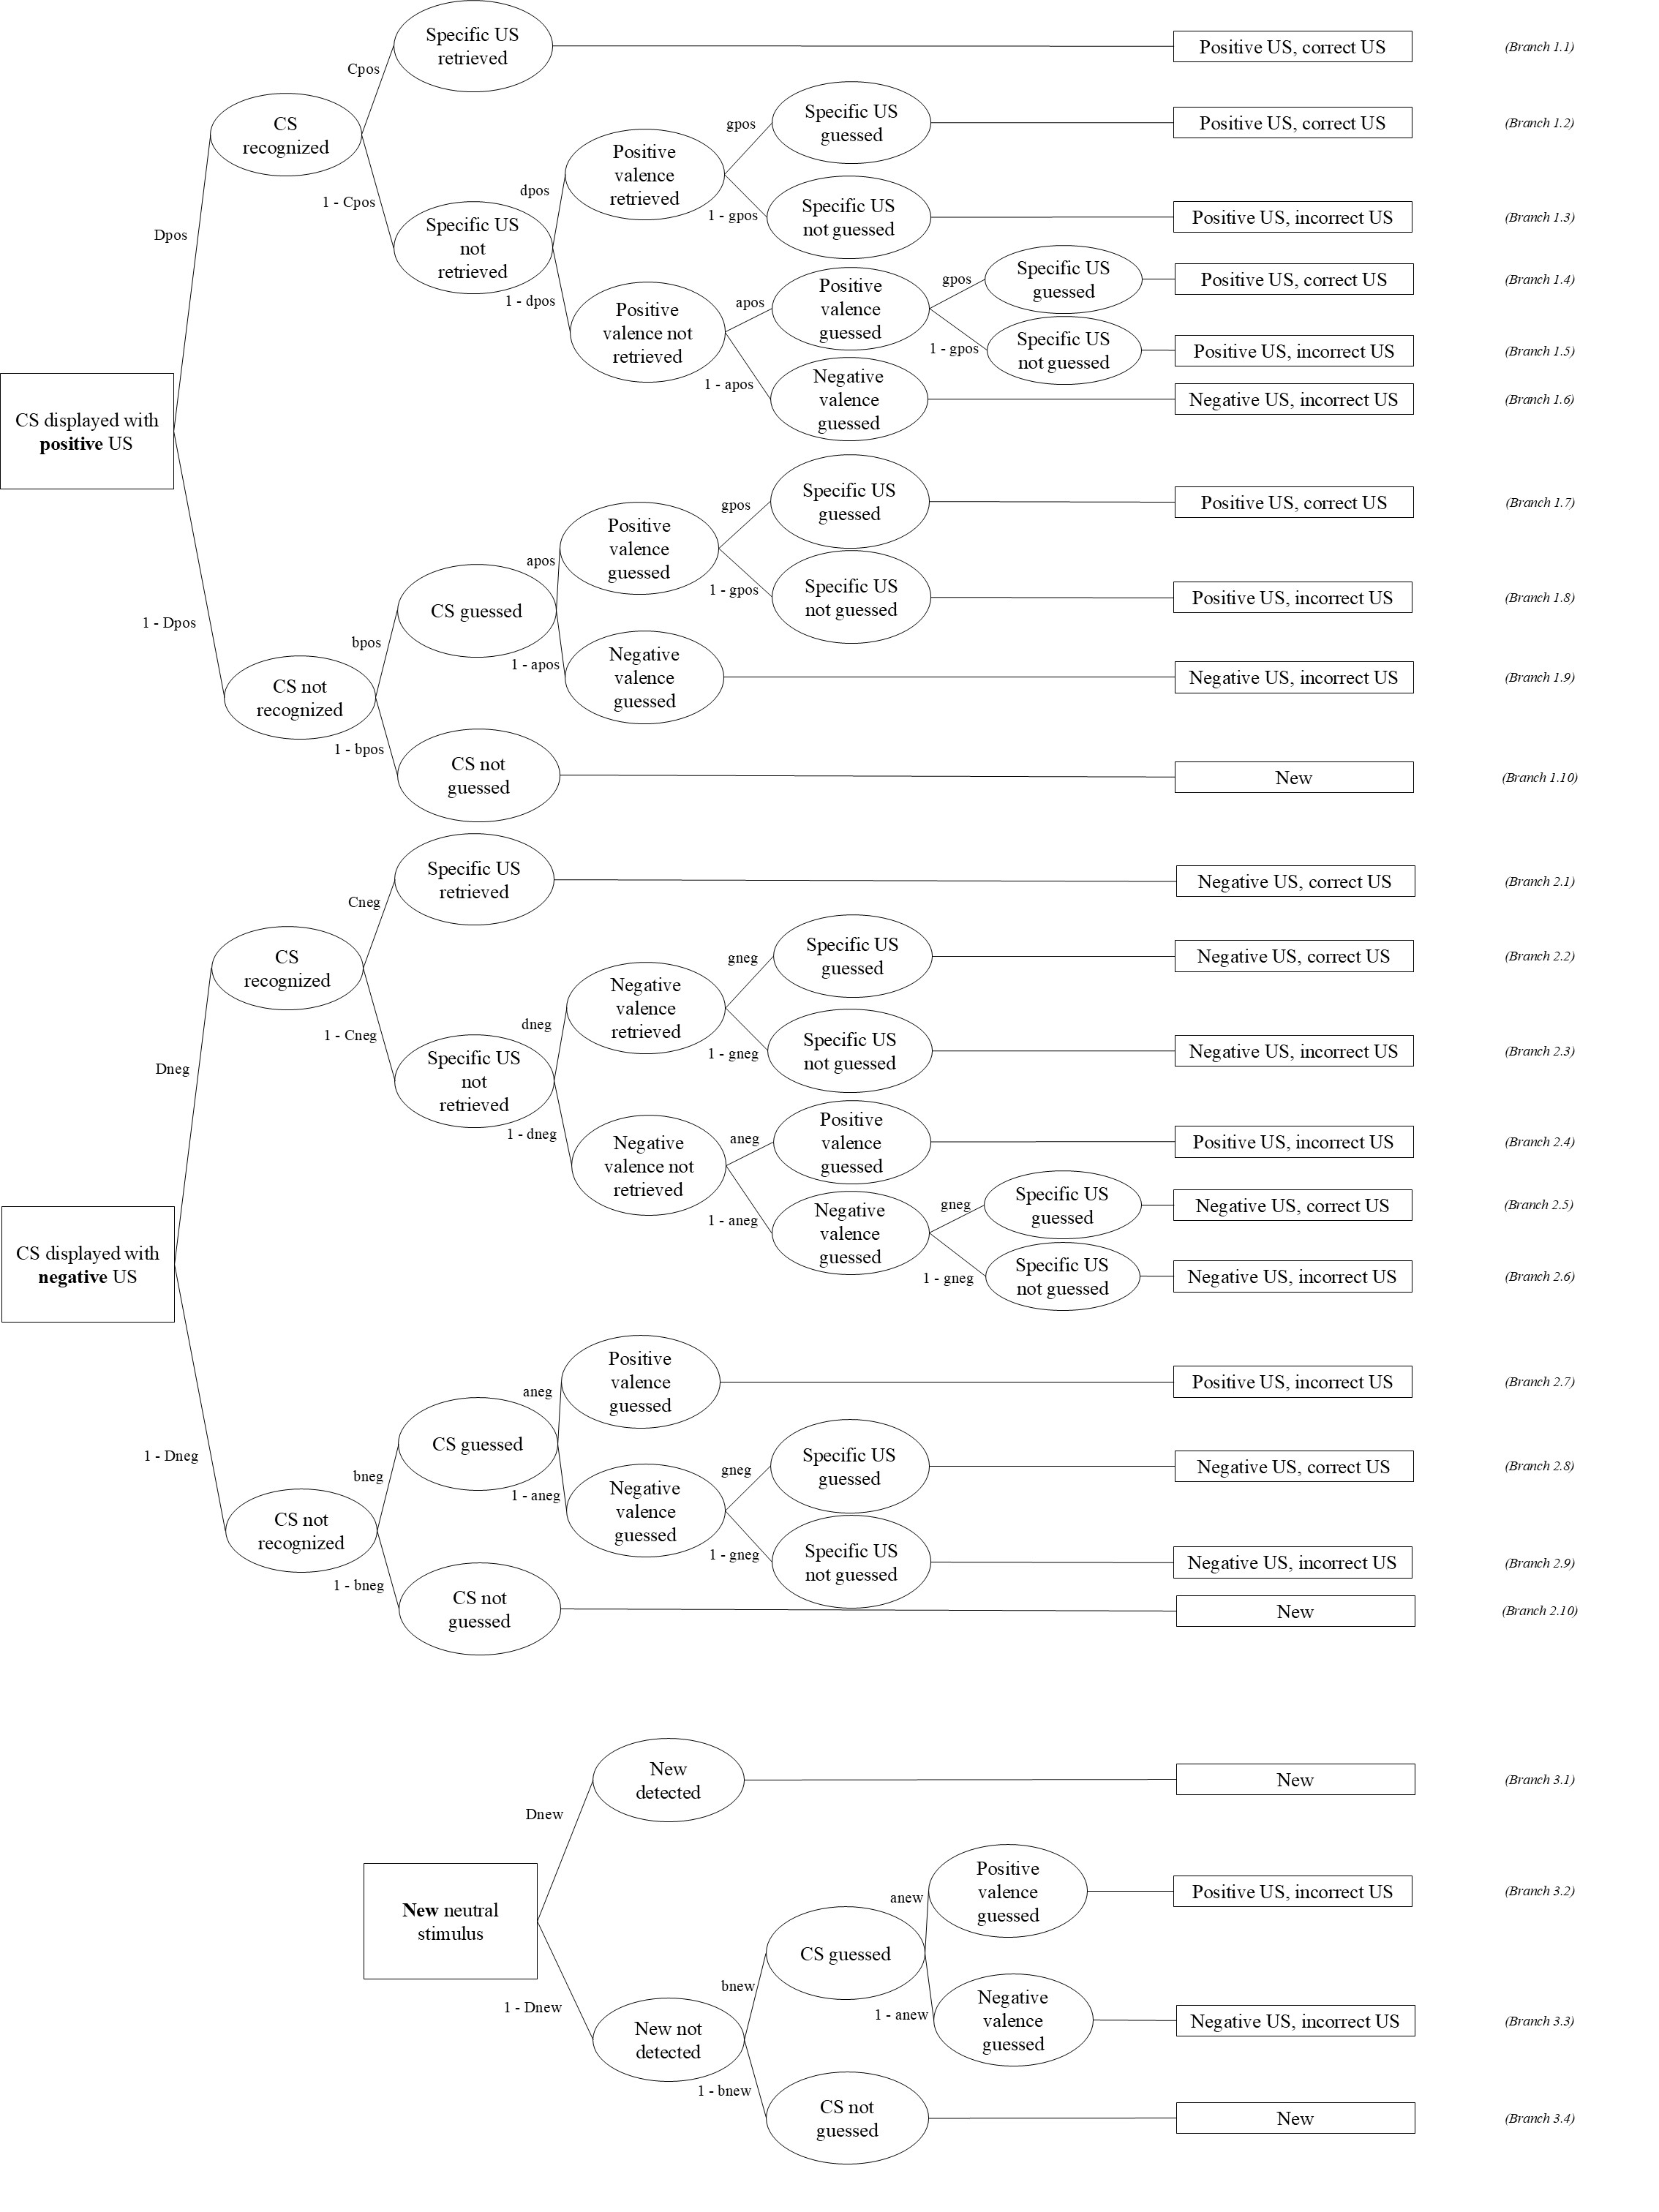
\includegraphics[width=7.56in]{mpt_wsw_model_exp3_KB2} \caption{The `who said what' multinomial processing tree model in the context of an evaluative conditioning procedure. The rectangles on the left-hand side represent the stimuli displayed in the memory task, and the rectangles on the right-hand side represent the responses.}\label{fig:cspos-tree}
\end{figure}

\subsection{Prior research and predictions}\label{prior-research-and-predictions}

The present study is a conceptual replication and extension of Gast and Rothermund (2011).
Gast and Rothermund (2011) showed that EC effects are moderated by the task that is performed during the learning procedure: across three experiments, EC effects were found to be stronger with tasks that focused on valence rather than on other, non-valent stimulus dimensions (e.g., age).
In the present experiment, we will implement the task focus manipulation from Gast and Rothermund's (2011) Experiment 2 (valence focus vs.~age focus), expecting to replicate the so-called valence focus effect on EC (prediction P1: \(\textrm{EC}_\textrm{valence-focus}>\textrm{EC}_\textrm{age-focus}\)).

In addition to boosting EC effects, valence focus tasks were also found to improve associative (in the present case, item-item) memory for the identity of the paired US as well as for the valence of the paired US (Gast \& Rothermund, 2011).
In the present experiment, we will test for similar effects of task focus on (associative) memory by comparing MPT parameter estimates between task focus conditions.
This model-based approach to testing these effects will overcome certain drawbacks in the methods used by Gast and Rothermund (2011) and provide more fine-grained insights into the effects of task focus on associative memory.

To measure associative memory for the US identity and for the US valence, Gast and Rothermund (2011) used a measurement procedure similar to the associative memory task that we will implement in the present experiment (i.e., selecting, for a given CS, the correct US from a list of positive and negative USs; see Experiments 1 and 3).
Based on this similarity, the drawbacks in the methods used by Gast and Rothermund (2011) can be illustrated by \emph{Figure 1}.
To quantify associative memory for the US valence, Gast and Rothermund (2011) calculated a CS-valence memory score indicating the number of CSs for which a US with the correct US valence was selected.
In the MPT model, this number corresponds to the sum of responses from branches \(1.1\), \(1.2\), \(1.3\), \(1.4\), \(1.5\), \(1.7\), \(1.8\), \(2.1\), \(2.2\), \(2.3\), \(2.5\), \(2.6\), \(2.8\) and \(2.9\) in Figure~\ref{fig:cspos-tree}.
From the perspective of the MPT model, differences in the CS-valence memory score (across task focus conditions) may therefore be driven by changes in any parameter contained in these 14 branches.
Since most of these parameters do not capture associative memory for the US valence, the CS-valence memory score used by Gast and Rothermund (2011) may thus yield artifactual evidence for an effect of task focus on this type of associative memory (most importantly, when the task focus manipulation affects associative memory for the US identity {[}as measured by the \(C\) parameters contained in branches \(1.1\) and \(2.1\){]} without affecting associative memory for the US valence {[}as measured by the \(d\) parameters contained in branches \(1.2\), \(1.3\), \(2.2\), and \(2.3\){]}).
A similar criticism applies to the CS-US memory score which was used by Gast and Rothermund (2011) to measure associative memory for the US identity.
The CS-US memory score was calculated as the number of CSs for which the correct US was selected, therefore corresponding to the sum of responses from branches \(1.1\), \(1.2\), \(1.4\), \(1.7\), \(2.1\), \(2.2\), \(2.5\), and \(2.8\) in Figure~\ref{fig:cspos-tree}.
As before, most parameters contained in these branches are unrelated to the to-be-measured type of associative memory, implying that the CS-US memory score may also yield artifactual evidence for a task focus effect on associative memory for the US identity (most importantly, when the task focus manipulation affects associative memory for the US valence {[}as measured by the \(d\) parameters contained in branches \(1.2\) and \(2.2\){]} without affecting associative memory for the US identity {[}as measured by the \(C\) parameters contained in branches \(1.1\) and \(2.1\){]}).

In the present experiment, we will avoid the previously mentioned confounds by testing for task focus effects on the \(C\) and \(d\) parameters estimated in the MPT model.
As explained earlier, the \(C\) parameter estimates the (conditional) probability of retrieving the correct US for a given CS recognized as coming from the learning phase (and may therefore de-confound task focus effects on US identity memory from effects on other forms of {[}associative{]} memory and/or on guessing processes).
Similarly, the \(d\) parameter estimates the (conditional) probability of retrieving the correct US valence (without retrieving the correct US identity) for a given CS recognized as coming from the learning phase (and may thus de-confound task focus effects on US valence memory from effects on other forms of {[}associative{]} memory and/or on guessing processes).
Based on a pilot study (in which we used the same materials and procedure), we expect significant task focus effects on both MPT parameters (prediction P2: \(C_\textrm{valence-focus}>C_\textrm{age-focus}\); prediction P3: \(d_\textrm{valence-focus}>d_\textrm{age-focus}\)).
Finally, we will also test for task focus effects on the \(D\), \(b\) and \(a\) parameters.
Based on the pilot study, we expect significant effects of task focus on the \(D\) and \(b\) parameters (prediction P4: \(D_\textrm{valence-focus}>D_\textrm{age-focus}\); prediction P5: \(b_\textrm{age-focus}>b_\textrm{valence-focus}\)).
For the \(a\) parameter, no such effect is expected.

\section{Methods}\label{methods}

\subsection{Design, participants and sample size}\label{design-participants-and-sample-size}

The experiment follows a 2 (\emph{US valence}: positive vs.~negative) \(\times\) 2 (\emph{US age}: young vs.~old) \(\times\) 2 (\emph{task focus}: valence focus vs.~age focus) mixed design.
The first two factors are varied within participants and the third factor is varied between participants.
Assignment to task focus conditions will be random (executed by the experimental software).

Participants will be recruited through Prolific and receive monetary compensation for participating in the study.
We do not commit to a specific sample size.
Instead, we pre-register a minimum sample size (per task focus condition), a maximum sample size (across task focus conditions), and two stopping criteria (determining the {[}dis-{]}continuation of data collection within the pre-registered sample size range).
In a first step, we will recruit participants until the minimum sample size\footnote{The minimum sample size per task focus condition is based on a power analyses for the two-way interaction between US valence and task focus. In this power analysis, we targeted a test power of \(1-\beta=.9\) and used an \(\alpha\)-level of \(.1\) to implement a one-tailed test of the two-way interaction (reflecting the directional prediction P1). The effect size of the US valence \(\times\) Task focus interaction was set to \(\eta^2_{p}\approx.079\) (corresponding, approximately, to one half of the effect size obtained in the pilot study).} is reached (52 non-excluded participants per task focus condition; exclusion criteria are listed below).
Based on this (minimum) sample, we will then fit the MPT model and calculate Bayes factors comparing a nested version of the model with \(d_\textrm{valence-focus}=d_\textrm{age-focus}\) to the baseline model with free \(d_\textrm{valence-focus}\) and \(d_\textrm{age-focus}\) (for details, see section ``Data processing and statistical analyses'').
The data collection will be discontinued at this point if (a) the Bayes factor in favor of the baseline model (free \(d_\textrm{valence-focus}\) and \(d_\textrm{age-focus}\)) exceeds 10 (i.e., if evidence for the presence of a task focus effect on the \(d\) parameter is strong) or (b)
the Bayes factor in favor of the nested version of the model (\(d_\textrm{valence-focus}=d_\textrm{age-focus}\)) exceeds 10 (i.e., if evidence for the absence of a task focus effect on the \(d\) parameter is strong).\footnote{The interpretation of a larger-than-ten Bayes factor as strong evidence (for the presence or absence of a task focus effect on the \(d\) parameter) is based on Lee and Wagenmakers (2014).}
If neither criterion is met, data collection will be continued in sets of 20 participants (excluded or non-excluded).
After each new set of 20 participants is collected, the previously mentioned Bayes factors will be calculated based on the total sample of non-excluded participants recruited so far.
As before, data collection will be discontinued after a given set of 20 participants if (a) the Bayes factor in favor of the baseline model (free \(d_\textrm{valence-focus}\) and \(d_\textrm{age-focus}\)) exceeds 10 or (b)
the Bayes factor in favor of the nested model (\(d_\textrm{valence-focus}=d_\textrm{age-focus}\)) exceeds 10.
If neither criterion is met, data collection will be continued in sets of 20 participants (excluded or non-excluded) until the maximum sample size\footnote{The maximum sample size was selected based on the financial resources available to the authors.} (200 participants in total) is reached.

\subsection{Materials}\label{materials}

The experiment is programmed with lab.js (Henninger, Shevchenko, Mertens, Kieslich, \& Hilbig, 2022) and exported to an HTTPS-protected website with JATOS (Lange, Kühn, \& Filevich, 2015).

The CS pool comprises 48 colored images of middle-aged human faces with neutral expressions (24 female faces, 24 male faces).
The images were taken from the FACES database (Ebner, Riediger, \& Lindenberger, 2010) and optimized with an AI image optimization tool.

The US pool comprises 24 adjectives describing human traits, with 6 adjectives in each US valence \(\times\) US age typicality condition.
Based on a pilot study, we selected six adjectives describing traits that are positive and more typical for younger (than for older) people (\emph{energetic}, \emph{flexible}, \emph{lively}, \emph{open-minded}, \emph{optimistic}, \emph{strong}), six adjectives describing traits that are positive and more typical for older (than for younger) people (\emph{calm}, \emph{dignified}, \emph{nurturing}, \emph{patient}, \emph{realistic}, \emph{wise}), six adjectives describing traits that are negative and more typical for younger (than for older) people (\emph{careless}, \emph{impulsive}, \emph{naive}, \emph{selfish}, \emph{spoilt}, \emph{self-absorbed}), and six adjectives describing traits that are negative and more typical for older (than for younger) people (\emph{demented}, \emph{feeble}, \emph{frail}, \emph{rigid}, \emph{stubborn}, \emph{weak}).

\subsection{Stimulus assignment}\label{stimulus-assignment}

For each participant, 12 randomly selected images of faces (half female, half male) will serve as positively paired CSs (i.e., they will be paired with a positive US during the learning phase), 12 randomly selected images of faces (half female, half male) will serve as negatively paired CSs (i.e., they will be paired with a negative US during the learning phase), and the remaining 24 images of faces (half female, half male) will serve as ``new'' stimuli (i.e., they will not be presented in the learning phase and appear only in the test phase).

For each participant, all 24 adjectives will serve as USs during the learning phase.
Each adjective will be randomly assigned to one of the 24 CSs. Six CSs (half images of female faces) will be paired with positive-typically young USs; 6 other CSs (half images of female faces) will be paired with positive-typically old USs; 6 other CSs (half images of female faces) will be paired with negative-typically young USs; the 6 last CSs (half images of female faces) will be paired with negative-typically old USs.

\subsection{Procedure}\label{procedure}

The study will be run online.
All verbal materials will be presented in English.
After providing their informed consent and being asked to focus on the study, participants will be thanked for their participation and asked to carefully read all instructions and perform the tasks. The instructions of the learning phase will then be presented.

\subsubsection{Learning phase}\label{learning-phase}

All participants will read the following instructions:
``In the first part of the experiment you will be presented with photographs of faces (called `faces' below) shown together with adjectives that denote human traits (called `traits' below).
Each face will be paired with a single trait.
For each face-trait pair, the trait will be presented first.
After a brief delay, the face will appear underneath.
Please pay close attention to all traits and faces.
Each face-trait pair will be presented for a limited time.
Your task will be to form an impression of each face-trait pair.''

Then, depending on the task focus condition (valence focus or age focus), participants will read:
``Specifically, you will have to indicate whether you think each face-trait pair is rather `negative' {[}`typically old'{]} or rather `positive' {[}`typically young'{]}.
Press the spacebar to continue with the instructions.''

The position of `negative', `positive', `typically old', and `typically young' labels will match the label key assignment used in the learning phase (randomly determined for each participant anew): `positive' (`typically old') on the A key and `negative' (`typically young') on the M key (or vice-versa).

The instructions will continue as follows:
``Next, you will be presented with the face-trait pairs.
Again, your task is to form an impression of each face-trait pair. You need to carefully look at both the faces and traits being presented.
Please indicate whether you think each pair is rather `negative' {[}`typically old'{]} or rather `positive' {[}`typically old'{]}.
If you think the pair is rather `negative' {[}`typically old'{]}, press `A' on your keyboard.
If you think the pair is rather `positive' {[}typically young'{]}, press `L' on your keyboard.
Although the presentation time is limited,
please try your best to provide a response on each face-trait pair.
This part of the experiment will take about 8 minutes.
When you are ready, press the spacebar to start the task.
(This may take a few seconds.)''

Again, the position of the `negative', `positive', `typically old', and `typically young' labels and the associated keys will match the label key assignment used in the learning phase.

Participants will then work through the learning task, consisting of 72 trials.
Each trial will start with a US presented alone in green lower-case letters against a black background at the top of the screen. After 1000 ms, the CS will appear right below the US.
The CS-US pair will remain on screen for 4000 ms.
Participants will have to respond within 3000 ms after the onset of the US (by pressing the ``A'' or ``L'' key).
If participants respond in time, three hyphens will appear below the CS-US pair right after participants have entered a response (to indicate that the response is recorded).
If participants do not respond in time (i.e., within the 3000 ms), the text ``no response'' will appear in red below the CS-US pair for 1000 ms.The CS-US pair will then disappear, and the message ``no response Press the spacebar to continue.'' will be displayed in red at the bottom of the screen without time limit.
The trials will be separated by an empty screen for 2500 ms.

For each participant, each CS-US pair will be presented once in a random order within each set of 24 CS-US pairs. Three CS-US pair sets will be presented. The CS-US pairs will be presented in a random order within each set.

After the learning phase, the following text will be displayed:
``The first part of the experiment is now finished!
You have now seen all face-trait pairs and may continue with the second part of the experiment.
Press the spacebar to continue.''

\subsubsection{Test phase}\label{test-phase}

Immediately after the learning phase, participants will enter the test phase. The test phase will be identical regardless of the task focus condition and label-key assignment in the learning phase. Participants will first perform an evaluative rating task and then a memory task.

\paragraph{Evaluative rating task}\label{evaluative-rating-task}

The evaluative rating task will be introduced as follows:
``In the second part of the experiment, you will be presented with individual faces.
Please indicate your personal evaluation of the presented faces.
To do so, you will be presented with an 8-point scale ranging from very negative (left) to very positive (right).
Please click on the scale point that best represents your evaluation of a given face.
When you are ready, press the spacebar to start the task.''.

Participants will then work through the evaluative rating task, consisting of 48 randomly ordered self-paced trials. On each trial, a face (one of the 24 CSs or one of the 24 new stimuli) will be presented in the upper half of the screen. In the lower half, the evaluation task question (``How negative or positive is your personal evaluation of the face presented above?'') together with a rating scale ranging from 1 (``very negative'') to 8 (``very positive'') will be displayed.
Trials will be separated by a blank screen presented for 500 ms.

At the end of the evaluative rating task, the following text will be displayed:
``The second part of the experiment is now finished.
Press the spacebar to continue with the third part.''

\paragraph{Memory task}\label{memory-task}

The memory task will be introduced as follows:
``In the third part of the experiment, you will again be presented with faces.
Some of these faces were part of the face-trait pairs you saw in the first part of this experiment.
Other faces were not shown in the first part of this experiment: these faces were not part of the face-trait pairs you saw in the first part of this experiment.
For each face, please indicate whether it is''shown'' (i.e., part of the face-trait pairs you saw) or
``not shown'' (i.e., NOT part of the face-trait pairs you saw).
Press the spacebar to continue with the instructions.''

On the next instruction slide, the following text will be displayed:
``Whenever you classify a face as `shown', you will be asked to perform a second task.
In this second task, you will be presented with 16 traits.
Your task will be to select the trait with which the face was paired in the first part of this experiment.
If you remember the paired trait, click on it.
If you cannot remember the previously paired trait, try to guess the correct one.
Click on the trait corresponding to your guess.
When you are ready, press the spacebar to start the task.''

Participants will then work through the memory task, consisting of 48 randomly ordered self-paced trials.
On each trial, an image (one of the 24 CSs or one of the 24 new stimuli) will be presented in the upper half of the screen.
In the lower half, the recognition task question (``Was this face part of the face-trait pairs you saw?'') together with the two response options ``Yes (shown)'' and ``No (not shown)'' will be displayed.
If participants respond ``No (not shown)'', they will see a blank screen (500 ms) and then proceed to the next trial (i.e., they will be presented with a screen showing another face, the recognition task question, and the two response options).
If participants respond with ``Yes (shown)'', they will see a blank screen (500 ms) and then proceed to the associative memory task.
For this task, the face will again be presented in the upper half of the screen.
In the lower half, the associative memory task question (``Which of the following traits was previously paired with the face presented above?'') together with 16 USs will be shown.
The 16 USs will be displayed as buttons organized in three rows (with six buttons in the upper two rows and four buttons in the bottom row).
For truly ``shown'' faces, the correct US will be presented on a randomly selected button, while the remaining buttons will be filled with 15 randomly selected USs that have been paired with other CSs.
Three of these USs will have the same US valence and US age as the correct US, four USs will have the same US valence but the opposite US age as the correct US, four USs will have the same US age but the opposite US valence as the correct US, and four USs will have the opposite US age and the opposite US valence as the correct US.
Other than that, the USs will be randomly selected for each trial and participant anew.
For new faces (erroneously classified as ``shown''), the buttons will be filled with 16 randomly selected USs (four USs per US valence \(\times\) US age condition). After clicking on one of the 16 USs, participants will be presented with a blank screen (500 ms) followed by the next trial (i.e., they will be presented with a screen showing another face, the recognition task question, and the two response options).

The end of the memory task will be announced by a slide showing the following text:
``The third and final part of the experiment is now finished.
Now we have a few short questions about your experience performing the study.
Press the spacebar to continue.''

\subsubsection{Check measures}\label{check-measures}

We will collect several check measures (which we will use as exclusion criteria).
First, participants will be presented with a screen showing four long sentences in a single paragraph.
The first three sentences will refer to attitude research and through length and writing style are meant to discourage participants from reading the whole text.
In the very last sentence of the text, participants will be instructed to ignore the upcoming question about their exercise habits (in order to demonstrate that they have read the entire passage).
On the next screen, participants will be presented with a list of seven physical activities and are asked to indicate which of these activities they performed regularly (by ticking a small box next to the respective activity).
After having ticked all relevant boxes (or none at all), participants proceed to the next screen by clicking on the ``Continue'' button displayed at the bottom of the screen.
Subsequently, participants will answer (``Yes'' or ``No'') the following attention check item: ``Did you pay attention to the faces and traits presented throughout the entire study? (the response to this question will not affect your payment.)''.
Next, participants will answer the following seriousness check (based on Aust, Diedenhofen, Ullrich, \& Musch, 2013): ``It would be very helpful if you could tell us at this point whether you have taken the requested responses seriously, so that we can use your answers for our scientific analysis, or whether you were just clicking through to take a look at the survey? (again, this will not affect your payment.)''.
The response options will be ``I have taken the requested responses seriously'' and ``I have just clicked through, please discard my data''.
Participants will then have the opportunity to share any comments and will be debriefed.

\subsection{Inclusion and Exclusion criteria}\label{inclusion-and-exclusion-criteria}

On Prolific Academic, sex will be balanced to have approximately the same proportions of male and female participants in our sample.
Moreover, we will only recruit participants (1) whose first language is English, (2) declaring to live in the USA or in the United Kingdom, (3) with an approval rate of at least 90\%, (4) with at least 20 previous submissions, and (5) who did not take part in previous pretests and experiments from members of the current team of authors conducted using the same materials.

Participants who fail at least one check measure (by selecting at least one physical activity, by responding with ``No'' to the attention check or by responding with ``I have just clicked through, please discard my data'' to the seriousness check) will be excluded from all analyses.
For individual analyses (on data from the evaluation, item and associative memory task), we will also exclude participants who gave the same response on all trials of the respective measurement procedure.

\subsection{Data processing and statistical analyses}\label{data-processing-and-statistical-analyses}

\subsubsection{Evaluative ratings}\label{evaluative-ratings}

For each participant, we will calculate an EC score by subtracting the mean evaluative rating for CSs presented with a negative US from the mean evaluative rating for CSs presented with a positive US.

Separated by task focus condition, we will test the mean EC score against zero (using one-sample \emph{t}-tests).
If the mean EC score is positive (indicating a regular EC effect), we will conduct a one-sided test (\(\alpha=.05\)).
If the mean EC score is negative, a two-sided test will be conducted (\(\alpha=.05\)).

To test prediction P1 (\(\textrm{EC}_\textrm{valence-focus}>\textrm{EC}_\textrm{age-focus}\)), we will conduct a two-sample \emph{t}-test comparing EC effects between task focus conditions.
If, in line with prediction P1, the mean EC score in the valence focus condition is numerically larger than the mean EC score in the age focus condition, we will conduct a one-sided test (\(\alpha=.05\)).
If the mean difference is reversed, a two-sided test will be conducted (\(\alpha=.05\)).
Note that the one-sided \emph{t}-test (with \(\alpha=.05\)) is an analogue of the \emph{F}-test (with \(\alpha=.1\)) for the two-way interaction of US valence and task focus (which was used to determine the minimal sample size).
For a direct match with the specifications of the power analyses, prediction P1 will also be tested in a 2 (US valence) \(\times\) 2 (task focus) mixed ANOVA on evaluative ratings (instead of EC scores).
As before, we will conduct a one-sided test of prediction P1 if the mean EC score in the valence focus condition is numerically larger than the mean EC score in the age focus condition (by using \(\alpha=.1\) for the two-way interaction between US valence and task focus).
If the mean difference is reversed, the significance of the two-way interaction will be judged based on \(\alpha=.05\).

\subsubsection{Memory data}\label{memory-data}

For each participant and CS, responses from the two memory tasks will be recoded into a joint memory index according to the following scheme.

\paragraph{CSs}\label{css}

\begin{itemize}
\item
  If a positively (negatively) paired CS is incorrectly classified as ``new'' in the recognition task, this response will be recoded as ``PosUSnew'' (``NegUSnew'') on the joint memory index.
\item
  If a positively (negatively) paired CS is correctly classified as ``old'' in the recognition task and the correct positive (negative) trait is chosen in the associative memory task, these responses will be recoded as ``PosUSposcor'' (``NegUSnegcor'') on the joint memory index.
\item
  If a positively (negatively) paired CS is correctly classified as ``old'' in the recognition task and an incorrect positive (negative) trait is chosen in the associative memory task, these responses will be recoded as ``PosUSposincor'' (``NegUSnegincor'') on the joint memory index.
\item
  If a positively (negatively) paired CS is correctly classified as ``old'' in the recognition task and a negative (positive) trait is chosen in the associative memory task, these responses will be recoded as ``PosUSnegincor'' (``NegUSposincor'') on the joint memory index.
\end{itemize}

\paragraph{New stimuli}\label{new-stimuli}

\begin{itemize}
\item
  If an (unpaired) new stimulus is correctly classified as ``new'' in the recognition task, the response will be recoded as ``Newnew'' on the joint memory index.
\item
  If an (unpaired) new stimulus is incorrectly classified as ``old'' in the recognition task and a positive (negative) trait is chosen in the associative memory task, these responses will be recoded as ``Newposincor'' (``Newnegincor'') on the joint memory index.
\end{itemize}

The frequency distribution of the joint memory index (aggregated across participants) will be analyzed with
a Bayesian implementation of the MPT model, which is available in the R packages TreeBUGS (Heck, Arnold, \& Arnold, 2018) and MPTmultiverse (Singmann, Heck, Barth, \& Aust, 2020; see also Singmann et al., 2024).
For each of the model's parameters, we will use (default) Beta priors with \(\alpha = \beta = 1\),
resulting in a uniform prior distribution in the unit interval.
We will use these default priors for both the baseline model and all nested versions of the model (see below).

We will first estimate a baseline model where parameters \(D\), \(C\), \(d\), \(a\) and \(b\) are free to vary between task focus conditions.
For both task focus conditions, the \(g\) parameter will be set to \(.125\) (corresponding to the inverse of the number of response options per US valence condition {[}8{]} in the associative memory task).
The baseline model thus includes the following invariance assumptions (within each task focus condition):

\begin{itemize}
\item
  (A1) \(D_\textit{pos}=D_\textit{neg}=D_\textit{new}\)
\item
  (A2) \(C_\textit{pos}=C_\textit{neg}\)
\item
  (A3) \(d_\textit{pos}=d_\textit{neg}\)
\item
  (A4) \(b_\textit{pos}=b_\textit{neg}=b_\textit{new}\)
\item
  (A5) \(a_\textit{pos}=a_\textit{neg}=a_\textit{new}\)
\item
  (A6) \(g_\textit{pos}=g_\textit{neg}=.125\)
\end{itemize}

To assess model fit, we will calculate the posterior-predictive fit statistic \(T_1\) (Klauer, 2010) together with its corresponding posterior-predictive \(p\) value.
We will interpret \(p \leq. 05\) as indicating insufficient model fit.

If the baseline model achieves adequate fit (i.e., \(p > .05\)),
we will estimate several restricted versions of the MPT model.
To test each parameter against its reference value (\(0\) for \(D\), \(C\) and \(d\); \(.5\) for \(a\) and \(b\); \(.125\) for \(g\)),
we will estimate separate models (each of which will include one of ten restrictions:
{[}1{]} \(D_\textrm{valence-focus}=0\),
{[}2{]} \(D_\textrm{age-focus}=0\),
{[}3{]} \(C_\textrm{valence-focus}=0\),
{[}4{]} \(C_\textrm{age-focus}=0\),
{[}5{]} \(d_\textrm{valence-focus}=0\),
{[}6{]} \(d_\textrm{age-focus}=0\),
{[}7{]} \(b_\textrm{valence-focus}=.5\),
{[}8{]} \(b_\textrm{age-focus}=.5\),
{[}9{]} \(a_\textrm{valence-focus}=.5\),
{[}10{]} \(a_\textrm{age-focus}=.5\)
and compare them with the unrestricted baseline model using the Bayes Factor.
To test for parameter differences between task focus conditions,
we will again estimate separate models (each of which will include one of five restrictions):
{[}11{]} \(D_\textrm{valence-focus}=D_\textrm{age-focus}\),
{[}12{]} \(C_\textrm{valence-focus}=C_\textrm{age-focus}\),
{[}13{]} \(d_\textrm{valence-focus}=d_\textrm{age-focus}\),
{[}14{]} \(b_\textrm{valence-focus}=b_\textrm{age-focus}\),
{[}15{]} \(a_\textrm{valence-focus}=a_\textrm{age-focus}\))
and compare these models against the baseline model using the Bayes Factor.

If the baseline model does not achieve adequate fit (i.e., \(p \leq .05\)),
we will try to identify a less restrictive (baseline) model that provides a more adequate account of the data.
Model selection (of an alternative baseline model) will be based on model comparisons using the Bayes Factor,
complemented by substantive and pragmatic considerations.
Such an alternative baseline model may eventually contain separate parameters for positive/negative/new stimuli (e.g., three separate \(D\) parameters \(D_\textit{pos}, D_\textit{neg}, D_\textit{new}\) within each task focus condition).
To test for differences between task focus conditions,
<<<<<<< HEAD
we will, accordingly, compare the alternative baseline model with more restrictive models setting one, two, or three of these parameters equal between task focus conditions (model comparisons will again be based on the Bayes Factor).
Note that the total number of restrictive models is determined by the number of possible parameters of a given type (\(D\): \(D_\textit{pos}\), \(D_\textit{neg}\), \(D_\textit{new}\); \(C\): \(C_\textit{pos}\), \(C_\textit{neg}\); \(d\): \(d_\textit{pos}\), \(d_\textit{neg}\); \(b\): \(b_\textit{pos}\), \(b_\textit{neg}\), \(b_\textit{new}\); \(a\): \(a_\textit{pos}\), \(a_\textit{neg}\), \(a_\textit{new}\); \(g\): \(g_\textit{pos}\), \(g_\textit{neg}\)).
=======
we will, accordingly, compare the alternative baseline model with more restrictive models setting one, two, or all of these three parameters equal between task focus conditions using the Bayes Factor.
>>>>>>> 285ba1fd5c01c9d846031fc56ad114b32e047600

\section{References}\label{references}

\phantomsection\label{refs}
\begin{CSLReferences}{1}{0}
\bibitem[\citeproctext]{ref-aust_seriousness_2013}
Aust, F., Diedenhofen, B., Ullrich, S., \& Musch, J. (2013). Seriousness checks are useful to improve data validity in online research. \emph{Behavior Research Methods}, \emph{45}(2), 527--535. \url{https://doi.org/10.3758/s13428-012-0265-2}

\bibitem[\citeproctext]{ref-ebner_facesdatabase_2010}
Ebner, N. C., Riediger, M., \& Lindenberger, U. (2010). {FACES}---{A} database of facial expressions in young, middle-aged, and older women and men: {Development} and validation. \emph{Behavior Research Methods}, \emph{42}(1), 351--362. \url{https://doi.org/10.3758/BRM.42.1.351}

\bibitem[\citeproctext]{ref-gast_what_2011}
Gast, A., \& Rothermund, K. (2011). What you see is what will change: {Evaluative} conditioning effects depend on a focus on valence. \emph{Cognition and Emotion}, \emph{25}(1), 89--110. \url{https://doi.org/10.1080/02699931003696380}

\bibitem[\citeproctext]{ref-heck_treebugs_2018}
Heck, D. W., Arnold, N. R., \& Arnold, D. (2018). {TreeBUGS}: {An R} package for hierarchical multinomial-processing-tree modeling. \emph{Behavior Research Methods}, \emph{50}(1), 264--284. \url{https://doi.org/10.3758/s13428-017-0869-7}

\bibitem[\citeproctext]{ref-henninger_labjs_2022}
Henninger, F., Shevchenko, Y., Mertens, U. K., Kieslich, P. J., \& Hilbig, B. E. (2022). Lab.js: {A} free, open, online study builder. \emph{Behavior Research Methods}, \emph{54}(2), 556--573. \url{https://doi.org/10.3758/s13428-019-01283-5}

\bibitem[\citeproctext]{ref-klauer_hierarchical_2010}
Klauer, K. C. (2010). Hierarchical {Multinomial Processing Tree Models}: {A Latent-Trait Approach}. \emph{Psychometrika}, \emph{75}(1), 70--98. \url{https://doi.org/10.1007/s11336-009-9141-0}

\bibitem[\citeproctext]{ref-klauer_unraveling_1998}
Klauer, K. C., \& Wegener, I. (1998). Unraveling social categorization in the '{Who} said what?' paradigm. \emph{Journal of Personality and Social Psychology}, \emph{75}(5), 1155--1178. \url{https://doi.org/10.1037/0022-3514.75.5.1155}

\bibitem[\citeproctext]{ref-lange_just_2015}
Lange, K., Kühn, S., \& Filevich, E. (2015). "{Just} another tool for online studies" ({JATOS}): {An} easy solution for setup and management of web servers supporting online studies. \emph{PloS One}, \emph{10}(6), e0130834. Retrieved from \url{https://journals.plos.org/plosone/article?id=10.1371/journal.pone.0130834}

<<<<<<< HEAD
\leavevmode\vadjust pre{\hypertarget{ref-lee_bayesian_2014}{}}%
Lee, M. D., \& Wagenmakers, E.-J. (2014). \emph{Bayesian cognitive modeling: {A} practical course}. New York, NY, US: Cambridge University Press. \url{https://doi.org/10.1017/CBO9781139087759}

\leavevmode\vadjust pre{\hypertarget{ref-singmann_mptmultiverse_2020}{}}%
=======
\bibitem[\citeproctext]{ref-lee_bayesian_2014}
Lee, M. D., \& Wagenmakers, E.-J. (2014). \emph{Bayesian cognitive modeling: {A} practical course}. New York, NY, US: Cambridge University Press. \url{https://doi.org/10.1017/CBO9781139087759}

\bibitem[\citeproctext]{ref-singmann_mptmultiverse_2020}
>>>>>>> 285ba1fd5c01c9d846031fc56ad114b32e047600
Singmann, H., Heck, D. W., Barth, M., \& Aust, F. (2020). \emph{{MPTmultiverse}: {Multiverse Analysis} of {Multinomial Processing Tree Models}}. \url{https://doi.org/10.32614/CRAN.package.MPTmultiverse}

\bibitem[\citeproctext]{ref-singmann_evaluating_2024}
Singmann, H., Heck, D. W., Barth, M., Erdfelder, E., Arnold, N. R., Aust, F., \ldots{} Groß, J. (2024). Evaluating the {Robustness} of {Parameter Estimates} in {Cognitive Models}: {A Meta-Analytic Review} of {Multinomial Processing Tree Models Across} the {Multiverse} of {Estimation Methods}. \emph{Psychological Bulletin}, \emph{150}(8), 965--1003. \url{https://doi.org/10.1037/bul0000434}

\end{CSLReferences}


\end{document}
